\documentclass[11pt,aspectratio=169,xcolor=dvipsnames, french]{beamer}
\usepackage[utf8]{inputenc}
\usepackage[francais]{babel} 
\usepackage[T1]{fontenc}
\usepackage{amsmath}
\usepackage{amsfonts}
\usepackage{amssymb}
\usepackage{graphicx}
\usepackage{multicol}
\usetheme{General}

\usepackage{xcolor}
%\usetheme{Montpellier}



\usepackage[ruled,lined]{algorithm2e}



\title{ADAM : Une méthode pour l'optimisation stochastique}
\author{Guillaume BERNARD-REYMOND, Guillaume BOULAND,\\ Camille MOTTIER, Abel SILLY}
\date{14 octobre 2024}

\setbeamertemplate{navigation symbols}{}
\setbeamertemplate{footline}[frame number]

\setlength\parindent{0cm}

\begin{document}

\frame{\titlepage}

\begin{frame}{L'article}
\begin{center}
 \textbf{Adam : A Method for Stochastic Optimization}

\begin{multicols}{2}

 Diederik P. Kingma\\
 {\small Université d'Amsterdam, OpenAI}
 
 \columnbreak
 
 Jimmy Lei Ba\\
 {\small Université de Toronto}
\end{multicols}

Première année de publication : 2014


\includegraphics[width=3cm]{ICLR_Logo.png}
\end{center}

\end{frame}

\begin{frame}{L'objectif}
	\begin{minipage}[c]{.4\linewidth}
$f(\theta)$ : fonction-objectif stochastique 

\

Exemple : $f(\theta)=\displaystyle\sum_{i=1}^{n}L(x_i|\theta)$ 

\

Mini-batch : $f_t(\theta)=\displaystyle \sum_{i\in I_t}L(x_i|\theta)$

\

Objectif : minimiser $\mathbb E[f(\theta)]$
	\end{minipage} \hfill
	\begin{minipage}[c]{.55\linewidth}
	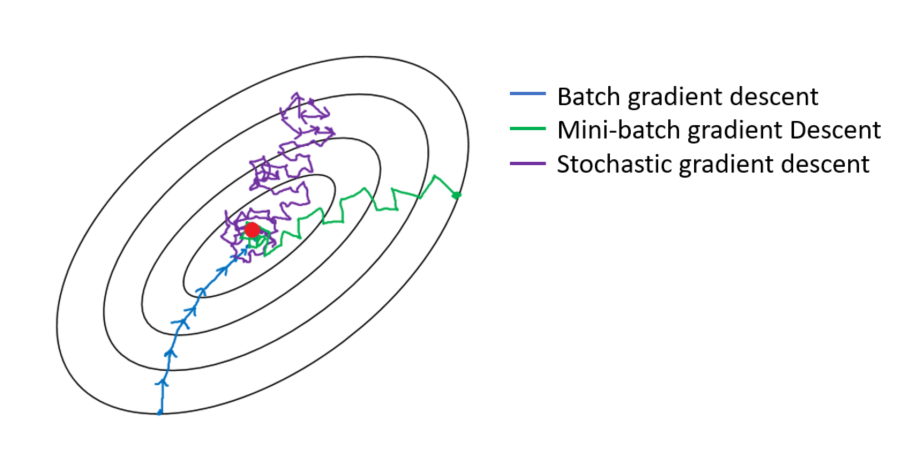
\includegraphics[width=8.5cm]{batch.png}

	\end{minipage}




\end{frame}

\begin{frame}{Méthode d'ordre 1}
Rappel : Qu'est-ce qu'une méthode d'ordre 1 ? Évaluation de $f(\theta)$ et de $\nabla_{\theta}f(\theta)$

\begin{center}
\scalebox{0.8}{
\begin{algorithm}[H]
  \caption{Descente de gradient stochastique}
  \Entree{$f(\theta)$, $\alpha$, $\theta_0$}
  $t\longleftarrow 0$ \\
  \Tq{$\theta_t$ ne converge pas}{
    $t\longleftarrow t+1$\\
    $g_t \longleftarrow \nabla_{\theta}f_t(\theta_{t-1})$\\
    $\theta_t \longleftarrow \theta_{t-1}-\alpha \cdotp g_t(\theta_{t-1})$
  }
  \Sortie{$\theta_t$}
\end{algorithm}}

\end{center}

\end{frame}

\begin{frame}{L'algorithme d'ADAM}
\begin{center}
\scalebox{0.9}{


\begin{algorithm}[H]
  \caption{Adam}
  \Entree{$f(\theta)$, $\alpha$, $\beta_1$, $\beta_2$, $\varepsilon$, $\theta_0$}
  $m_0\longleftarrow 0$ \\
  $v_0\longleftarrow 0$ \\  
  $t\longleftarrow 0$ \\
  \Tq{$\theta_t$ ne converge pas}{
    $t\longleftarrow t+1$\\
    $g_t \longleftarrow \nabla_{\theta}f_t(\theta_{t-1})$\\
    $m_t \longleftarrow \beta_1\cdotp m_{t-1}+(1-\beta_1)\cdotp g_t$ \hspace{2cm}( Estimateur de $\mathbb E[g_t]$ )\\
    \invisible {$v_t \longleftarrow \beta_2\cdotp v_{t-1}+(1-\beta_2)\cdotp g_t^2$
    \hspace{2.2cm}( Estimateur de $\mathbb E[g_t^2]$ )
    }\\
    \invisible {$\widehat m_t \longleftarrow m_t/(1-\beta_1^t)$\hspace{4cm}( \og débiaisage \fg{} )}\\
    \invisible {$\widehat v_t \longleftarrow v_t/(1-\beta_2^t)$}\\
    \invisible {$\theta_t \longleftarrow \theta_{t-1}-\alpha\cdotp \widehat m_t/(\sqrt{\widehat v_t}+\varepsilon)$\hspace{2.2cm}( Mise à jour )}
  }
  \Sortie{$\theta_t$}
\end{algorithm}
}
\end{center}
\end{frame}

\begin{frame}
 Illustartion  Guibou !
\end{frame}



\begin{frame}{L'algorithme d'ADAM}
\begin{center}
\scalebox{0.9}{


\begin{algorithm}[H]
  \caption{Adam}
  \Entree{$f(\theta)$, $\alpha$, $\beta_1$, $\beta_2$, $\varepsilon$, $\theta_0$}
  $m_0\longleftarrow 0$ \\
  $v_0\longleftarrow 0$ \\  
  $t\longleftarrow 0$ \\
  \Tq{$\theta_t$ ne converge pas}{
    $t\longleftarrow t+1$\\
    $g_t \longleftarrow \nabla_{\theta}f_t(\theta_{t-1})$\\
    $m_t \longleftarrow \beta_1\cdotp m_{t-1}+(1-\beta_1)\cdotp g_t$ \hspace{2cm}( Estimateur de $\mathbb E[g_t]$ )\\
    $v_t \longleftarrow \beta_2\cdotp v_{t-1}+(1-\beta_2)\cdotp g_t^2$
    \hspace{2.2cm}( Estimateur de $\mathbb E[g_t^2]$ )
    \\
    \visible<2-3> {$\widehat m_t \longleftarrow m_t/(1-\beta_1^t)$\hspace{4cm}( \og débiaisage \fg{} )}\\
    \visible<2-3> {$\widehat v_t \longleftarrow v_t/(1-\beta_2^t)$}\\
    \visible<3> {$\theta_t \longleftarrow \theta_{t-1}-\alpha\cdotp \widehat m_t/(\sqrt{\widehat v_t}+\varepsilon)$\hspace{2.2cm}( Mise à jour )}
  }
  \Sortie{$\theta_t$}
\end{algorithm}
}
\end{center}
\end{frame}

% \begin{frame}{Explications}
% 
% $f_1,\ldots, f_T$ : fonction $f$ restreinte à des mini-batches aléatoires \\
% 
% \pause
% 
% $g_t \longleftarrow \nabla_{\theta}f_t(\theta_{t-1})$ : mise à jour du gradient \\
% 
%  \pause
%  
% $\left.
% \begin{array}{ll}
%  m_t \longleftarrow \beta_1\cdotp m_{t-1}+(1-\beta_1)\cdotp g_t \\  
% v_t \longleftarrow \beta_2\cdotp v_{t-1}+(1-\beta_2)\cdotp g_t^2   
% \end{array}
% \right\rbrace$ : mise à jour des moments d'ordre 1 et 2 par moyenne mobile \\
% 
% 
%  
%  
% 
% \pause
% 
% $\left.
% \begin{array}{ll}
% \widehat m_t \longleftarrow m_t/(1-\beta_1^t) \\ 
%   \widehat v_t \longleftarrow v_t/(1-\beta_2^t)      
% \end{array}
% \right\rbrace$ : débiaisage des moments d'ordre 1 et 2 
% 
%  \pause
% 
%  $\theta_t \longleftarrow \theta_{t-1}-\alpha\cdotp \widehat m_t/(\sqrt{\widehat v_t}+\varepsilon)$ : Mise à jour de $\theta_t$
%  
%  changer la forme : moche
% 
% \end{frame}
% 
% \begin{frame}{Mise à jour des paramètres}
% $\alpha,\beta_1,\beta_2$
% \end{frame}

\begin{frame}{Biais}
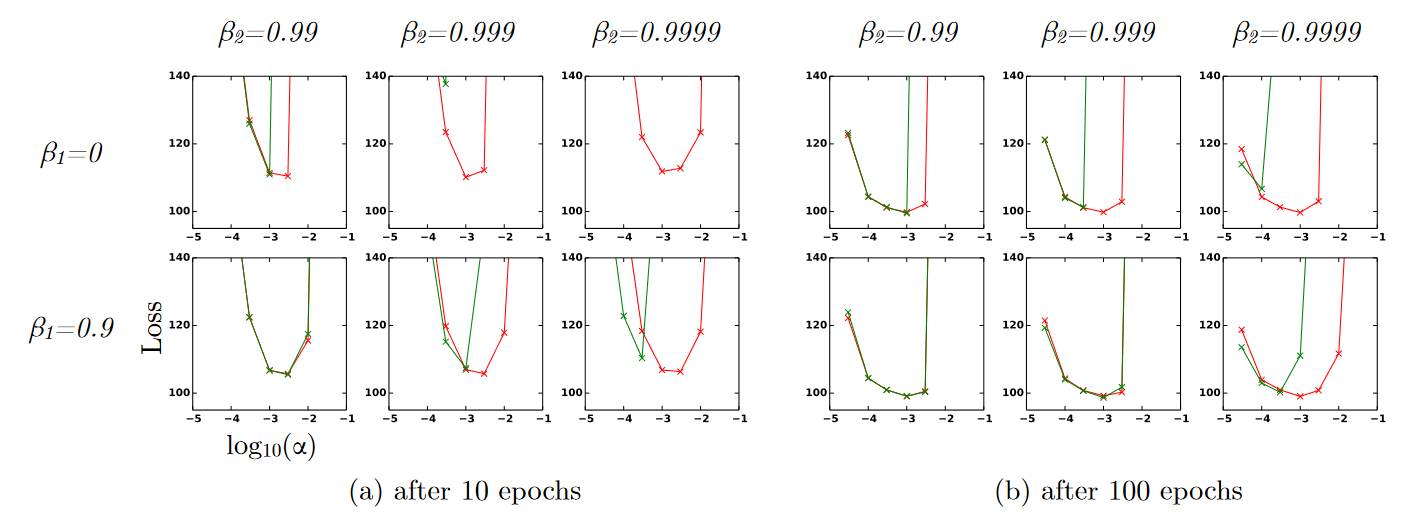
\includegraphics[width=\linewidth]{../Images/bias_correction_article.png}

mettre que pour 100 epochs ? rouge/vert : peu visible
\end{frame}

\begin{frame}{Résultats de convergence}

On définit le regret par : $$R(T)=\sum_{t=1}^{T}f_t(\theta_t)-\min_{\theta\in\mathcal{X}}\sum_{t=1}^{T}f_t(\theta)$$

\begin{theorem}
  Sous certaines hypothèses de majoration du gradient de $f_t$, et de l'écart entre les valeurs de $\theta_n$ on a : 
    $$\frac{R(T)}{T}=O\left(\frac{1}{\sqrt{T}}\right)$$  
\end{theorem}

\end{frame}



\begin{frame}{Simulations numériques}
  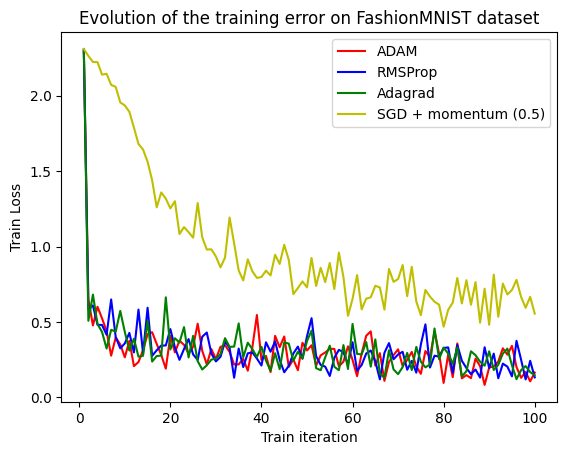
\includegraphics[width=0.45\linewidth]{../Images/FashionMNIST.png} \hfill 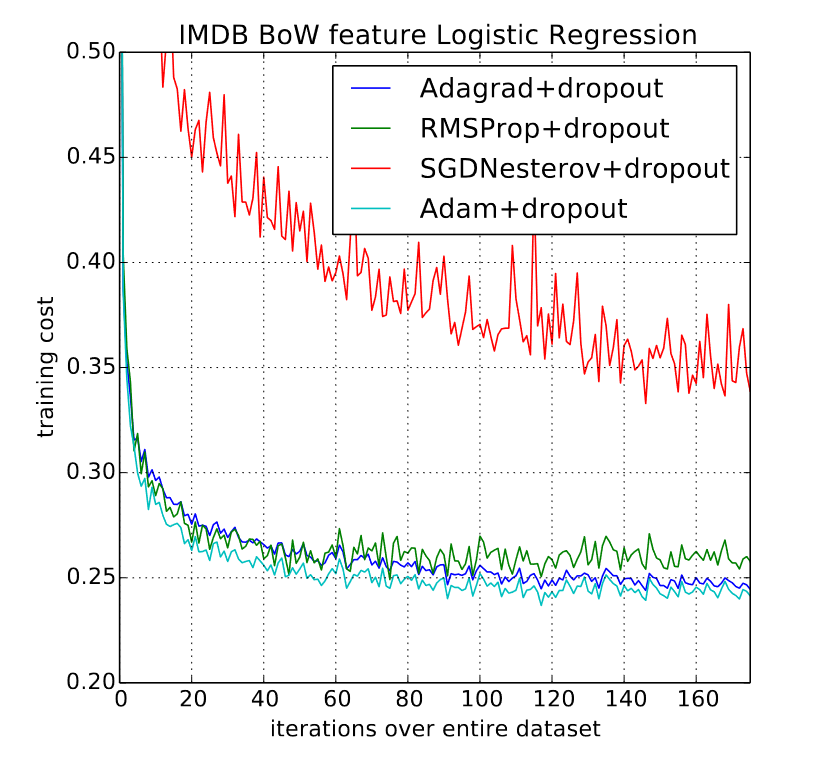
\includegraphics[width=0.45\linewidth]{../Images/IMDB_article.png}
\end{frame}

\begin{frame}{Conclusion}
ADAM est un algorithme :  

\begin{itemize}
\item[$\bullet$] facilement implémentable 
\item[$\bullet$] peu gourmand en mémoire
\item[$\bullet$] efficace dans de nombreux cas
\end{itemize}

D'où son succès !! 

Limite de l'article : manque de support théorique

\end{frame}

\end{document}
